\section{Static Single Assignment}

In this lecture we will cover what is SSA and how to convert a program to SSA form.

\subsection{}

When we are trying to do some types of optimizations, it is often nice to know when is a variable is defined.
For loop invariant code motion where we are trying to move computations outside of a loop, you will see it is very important to 
know where the definitions are.



Take the code for example, 

\begin{figure}[h]
    \centering
    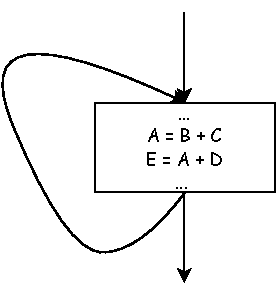
\includegraphics[width=0.4\textwidth]{ssaexm1.drawio.pdf}
    \caption{Example of Loop-Invariant Code Motion}
    \label{fig:ssaexm1}
\end{figure}




\subsection{The Development of Static Single Assignment Form}

This concept is based on \footnote{\url{https://compilers.cs.uni-saarland.de/ssasem/talks/Kenneth.Zadeck.pdf}}


In the very Beginning, there was dataflow analysis.   Ultimately dataflow analysis turns out to be very expensive.

Viewing the program variable by variable exposes structure that is obscured by the dataflow model: 
A kill allows the cfg to be clipped. Also, the dataflow for a single variable can be solved
without iteration. This turns out to be a dead end, but it set the
stage for the development of SSA.


Take constant propogation for example, Kildall and Wegbreit use a conventional
dataflow framework. The fact vector is very large: values not bits. Must use iteration.
The time to run these is between \(O(ElogEV)\) and
\(O(E^2 V)\) depending on the type of control flow
graph processing.



\subsubsection{The First Attack}


Use def-use chains. Sometimes this helps and sometimes it does not. This requires NMV
def-use chains.

\begin{lstlisting}[language=C,frame=single, caption=An ,label = lst:expr2]
switch (...) {
case 1: x=...; y=...; break;
...
case n: x=...; y=...; break;
}
switch (...) {
case 1: ...=x; ...=y; break;
...
case m: ...=x; ...=y; break;
}
\end{lstlisting}


\subsubsection{The Second Attack }


Add a “join birthpoint”
for x and y between
the two switches. 



\begin{lstlisting}[language=C,frame=single, caption=An ,label = lst:expr2]
    switch (...) {
    case 1: x=...; y=...; break;
    ...
    case n: x=...; y=...; break;
    }
    birthpoint x, y;
    switch (...) {
    case 1: ...=x; ...=y; break;
    ...
    case m: ...=x; ...=y; break;
    }
    \end{lstlisting}